\documentclass[12pt]{article}

\usepackage{etoolbox}
\usepackage{sbc-template}
\usepackage{graphicx,url}
\usepackage[utf8]{inputenc}
\usepackage[brazil]{babel}
\usepackage[none]{hyphenat}
\usepackage{amsmath}
\usepackage{amssymb} 
\usepackage{float}

\makeatletter
\patchcmd{\@startsection}
{\@afterindentfalse}
{\@afterindenttrue}
{}{}
\makeatother
     
\sloppy

\title{Cobertura e Acessibilidade: Aplicação de P-Médianas e PLMC em um Recorte Urbano}

\author{Anthony França, Antônio Neto, Enzo Santana, Franck Vasconcelos,\\
Murilo Mota, Rafael Gonçalves, Rene Marinho}

\address{Universidade Tiradentes (UNIT)\\}
\date{2025}

\begin{document} 

\maketitle
     
\begin{resumo}
Este estudo apresenta um panorama das principais formulações dos Problemas de Localização de Instalações (Facility Location Problems — FLPs) e suas aplicações em contextos urbanos. Apresenta-se um cenário ilustrativo que compara duas formulações clássicas: o Problema das P-Medianas e o Problema de Localização de Máxima Cobertura (PLMC). Descrevem-se as metodologias empregadas para cada variante e discutem-se as implicações práticas e as limitações de uma análise exploratória baseada em dados abertos, destacando como diferentes abordagens servem a objetivos distintos, reduzir deslocamentos médios ou ampliar a cobertura territorial.
\end{resumo}

\section{Introdução}

O posicionamento ideal de instalações é crucial para a provisão eficiente de serviços, sejam eles de natureza comercial ou pública, assim como para a integração regional por meio de infraestruturas físicas, como pontes, aeroportos e terminais rodoviários. No âmbito da Pesquisa Operacional, esse desafio é tratado pelo Problema de Localização de Instalações (PLI), cujo objetivo é selecionar locais de instalação que maximizem o atendimento à demanda e a acessibilidade dos usuários. Tais decisões devem considerar critérios diversos, como a maximização da cobertura da demanda, a minimização dos custos operacionais e a garantia de níveis mínimos de atendimento para determinados grupos de clientes (Sousa Filho et al., 2012; Rushton, 1979).

Várias formulações matemáticas têm sido propostas para atender a esses objetivos, destacando-se, entre elas, o Problema de Localização de Máxima Cobertura (PLMC) e o Problema das P-Medianas. Esses modelos dependem de fatores como a distribuição geográfica da população e os tempos de deslocamento para determinar soluções viáveis e eficientes. De fato, estudos recentes apontam que esses critérios de localização buscam garantir a acessibilidade, ponderando simultaneamente a demanda por serviços e as distâncias de viagem (Kuo e Kung, 2025).

Entre os cenários de aplicação dos PLI, destaca-se a relação entre instalações e clientes. Quando a instalação a ser aberta é escolhida dentre um conjunto de locais potenciais e os clientes são alocados a essas instalações visando minimizar o custo total de atendimento à demanda, obtém-se a formulação conhecida como Problema de Localização de Instalações sem Limitação de Capacidade (Uncapacitated Facility Location Problem - UFLP). Por outro lado, quando as demandas dos clientes devem ser atendidas exclusivamente por instalações com capacidade limitada, sem possibilidade de fracionar a demanda entre diferentes locais, o problema é classificado como o Problema de Localização de Instalações Capacitado de Fonte Única (Single-Source Capacitated Facility Location Problem - CFLP).

Tanto o UFLP quanto o CFLP baseiam-se na minimização dos custos de transporte entre clientes e instalações, desconsiderando fatores subjetivos, como a preferência dos usuários por determinada instalação (o que pode influenciar sua propensão a utilizá-la). Nesse contexto, esses problemas assumem caráter NP-difícil, uma vez que é necessário considerar numerosas combinações de alocação de clientes a instalações (Kang et al., 2023; Büsing et al., 2024).

Grande parte das formulações propostas adota cenários determinísticos, nos quais variáveis de demanda e tempo de viagem são tratadas como valores fixos. No entanto, dada a natureza NP-difícil desses problemas, surgem limitações inerentes na busca por soluções ótimas. Mesmo os modelos clássicos, que fornecem descrições generalistas adequadas, apresentam restrições significativas em contextos de alta incerteza ou dinamicidade, que poderiam refletir de forma mais realista a complexidade dos cenários reais. Incertezas e aspectos dinâmicos podem ser incorporados aos modelos de localização por meio de ferramentas como programação estocástica e análise de cenários (Owen e Daskin, 1998).

A seguir, são apresentadas considerações sobre a motivação e os objetivos deste trabalho. Em seguida, traçaremos um panorama dos principais estudos na área de localização de instalações, enfatizando os trabalhos mencionados (especialmente a metodologia de análise utilizada por Rushton e a revisão de Owen e Daskin). Posteriormente, na seção de Fundamentação Teórica, descreveremos as formulações adotadas para os problemas estudados, e, por fim, nas seções de Metodologia e Resultados, detalharemos os procedimentos adotados na análise do cenário.

\subsection{Importância do tema}

Os problemas de localização de instalações constituem um campo consolidado de pesquisa, com aplicações que variam desde estudos descritivos da infraestrutura existente até modelos preditivos para o planejamento futuro. Apesar das dificuldades inerentes à simulação de múltiplos cenários reais, em particular quando os dados são limitados ou apresentam incerteza, esse arcabouço teórico oferece ferramentas úteis para analisar a relação entre oferta de serviços e padrões espaciais de demanda.  

No presente trabalho, ainda que de forma simplificada e exploratória, procedeu-se à extração e ao tratamento de dados abertos (OpenStreetMap). Essas operações possibilitaram gerar representações cartográficas e indicadores básicos de acessibilidade e cobertura. Assim, a relevância prática deste exercício reside na sua capacidade de transformar dados geoespaciais disponíveis em evidências interpretáveis que podem subsidiar reflexões e decisões de planejamento urbano preliminares.

\subsection{Objetivos}

O objetivo deste estudo foi conduzir uma análise exploratória, baseada em métodos clássicos de localização de instalações, para examinar a distribuição espacial das farmácias no bairro Centro de Aracaju, a partir de dados extraídos do OpenStreetMap. Mais especificamente, os objetivos realizados foram:

\begin{itemize}
    \item obter e preparar dados geoespaciais do OSM relativos às farmácias do bairro;
    \item gerar mapas de localização e faixas de cobertura para pedestres, raio de 400\,m, e analisar qualitativamente a sobreposição e as lacunas de cobertura observadas;
    \item ilustrar, de maneira conceitual, o comportamento esperado de duas formulações clássicas: o Problema das P-Medianas e o Problema de Localização de Máxima Cobertura (PLMC).
\end{itemize}

Ressalta-se que o objetivo não incluiu a realização de otimizações numéricas exaustivas nem a modelagem estocástica da demanda; ao invés disso, priorizou-se uma abordagem pragmática e descritiva, adequada ao caráter exploratório do estudo e à disponibilidade dos dados utilizados.

\section{Trabalhos Relacionados}

Segundo Owen e Daskin (1998), a teoria da localização de instalações teve início em 1909 com o trabalho pioneiro de Alfred Weber, que buscava posicionar um depósito de modo a minimizar a distância total até os clientes. Rushton (1978) descreve esses primeiros esforços como essencialmente analíticos e restritos a formulações matemáticas básicas e representações gráficas rudimentares, com aplicação prática limitada. Somente na década de 1960, com o advento da computação, pesquisadores puderam propor métodos aplicáveis a cenários reais de localização. Mesmo assim, as formulações clássicas mantiveram-se estáticas e determinísticas, considerando parâmetros de demanda e tempos de deslocamento como dados fixos, o que restringe sua flexibilidade diante de condições variáveis.

Estudos mais recentes têm buscado expandir essas abordagens tradicionais, incorporando conceitos de modularidade e dinamicidade. Alarcon-Gerbier e Buscher (2022) ressaltam que a modularidade, viabilizada por meio de unidades de produção realocáveis ou expansíveis e instalações móveis, vem recebendo atenção crescente, com aplicações emergentes em diversos setores. De modo similar, Kang et al. (2023) propuseram um modelo de localização de serviços que considera as preferências dos clientes pelas instalações, além de levar em conta explicitamente as capacidades das unidades, evidenciando a complexidade adicional introduzida por esses fatores. Nesses modelos modernos, pesquisadores ponderam não apenas os custos de transporte e a cobertura da demanda, mas também escolhas comportamentais dos usuários, ampliando os requisitos de viabilidade do sistema.

As primeiras proposições forneceram uma base conceitual sólida, porém restrita a cenários ideais de operação e atendimentos simplificados. Com o avanço da área, passaram a ser considerados contextos mais complexos, como interrupções no sistema. Um exemplo interessante é o estudo de Ramshani et al. (2019), que aborda um modelo de localização de dois níveis (Two-Level UFLP) sob incertezas de disrupção. Os autores desenvolvem formulações matemáticas e heurísticas para lidar com paralisações em pontos da rede, demonstrando como essas descontinuidades afetam a seleção de locais e as alocações. Esses avanços ilustram a tendência atual de modelagem mais realista dos problemas de localização, incorporando aspectos de resiliência operacional e logística associada às instalações.

\section{Fundamentação Teórica}

Os problemas de localização de instalações envolvem a decisão de designar uma ou mais unidades para atender a um determinado contexto. Como a formulação matemática não admite soluções fracionárias, por exemplo, “meia instalação”, tais problemas são tradicionalmente modelados por meio da Programação Inteira, em que as variáveis assumem valores inteiros e representam decisões binárias de abertura ou não de uma instalação.

Segundo Owen e Daskin (1998), embora a Programação Inteira seja a base predominante das formulações clássicas, essas abordagens costumam ser estáticas e determinísticas, pois não consideram explicitamente as incertezas do ambiente real, o que limita sua aplicabilidade em contextos dinâmicos ou sujeitos a variações imprevistas. Nessas circunstâncias, embora matematicamente consistentes, as soluções obtidas podem não refletir integralmente a complexidade prática do problema.

Como alternativas, Owen e Daskin (1998) sugerem métodos dinâmicos e estocásticos. Os métodos dinâmicos são indicados quando o cenário presente é conhecido, mas há interesse em projetar soluções para períodos futuros, considerando possíveis alterações no sistema. Já os métodos estocásticos permitem modelar explicitamente a incerteza, ao incorporar variáveis aleatórias relacionadas a fatores como demanda, custos e tempos de viagem. Nesse caso, a solução do problema busca identificar a localização ótima das instalações por meio de avaliações probabilísticas das variáveis ou da análise de cenários alternativos, caracterizando um modelo de planejamento baseado em cenários.

Neste trabalho, serão desenvolvidas análises fundamentadas em duas formulações clássicas da literatura: o Problema das P-Medianas, formulado por Hakimi (1964), e o Problema de Localização de Máxima Cobertura (PLMC), descrito por Church e ReVelle (1976). O Problema das P-Medianas consiste em alocar instalações de modo a minimizar o tempo médio de deslocamento entre cada cliente e a instalação que o atende. Nesse contexto, a formulação busca identificar posições ideais de instalações de forma que a acessibilidade seja maximizada e os custos de deslocamento sejam reduzidos ao mínimo possível. A formulação matemática do problema das P-Medianas pode ser expressa como um modelo de Programação Inteira da seguinte forma:
\[
\begin{aligned}
i \in I\ (I=\{1,\ldots,n\}) &\quad \text{índice/conjunto de clientes},\\
j \in J\ (J=\{1,\ldots,m\}) &\quad \text{índice/conjunto de instalações potenciais},\\
c_{ij} \ge 0 &\quad \text{custo/distância entre o cliente $i$ e a instalação $j$},\\
P \in \mathbb{Z}_{+} &\quad \text{número de instalações a serem abertas}.
\end{aligned}
\]
\[
x_{ij} =
\begin{cases}
1, & \text{se o cliente $i$ é atendido pela instalação $j$},\\
0, & \text{caso contrário},
\end{cases}
\quad
y_{j} =
\begin{cases}
1, & \text{se a instalação $j$ é aberta},\\
0, & \text{caso contrário}.
\end{cases}
\]
\begin{alignat*}{2}
\text{Minimizar}\quad 
& \sum_{i \in I}\sum_{j \in J} c_{ij}\,x_{ij} \\
\text{sujeito a}\quad
& \sum_{j \in J} x_{ij} = 1,                 && \quad \forall i \in I, \\
& \sum_{j \in J} y_{j} = P,                  && \\
& x_{ij} \le y_{j},                          && \quad \forall i \in I,\ \forall j \in J, \\
& x_{ij} \in \{0,1\},                        && \quad \forall i \in I,\ \forall j \in J, \\
& y_{j} \in \{0,1\},                         && \quad \forall j \in J.
\end{alignat*}

O PLMC, por sua vez, busca localizar um número limitado de instalações para maximizar a cobertura da demanda em uma distância máxima \(d\). Diferentemente do problema das P-Medianas, que objetiva minimizar as distâncias médias de deslocamento, o PLMC considera que um cliente está coberto se estiver a uma distância aceitável \(d\) de pelo menos uma instalação. Assim, a formulação prioriza atender o maior número possível de clientes (ou demanda) dentro de um raio \(d\), dado um número \(P\) de instalações a serem abertas.

\[
\begin{aligned}
w_i \ge 0 &\quad \text{demanda do cliente } i,\\
d_{ij} \ge 0 &\quad \text{distância entre o cliente $i$ e a instalação $j$},\\
P \in \mathbb{Z}_{+} &\quad \text{número de instalações a serem abertas},\\
d \ge 0 &\quad \text{distância máxima de cobertura}.
\end{aligned}
\]
Definem-se as variáveis:
\[
z_i = 
\begin{cases}
1, & \text{se o cliente $i$ está coberto por alguma instalação}, \\
0, & \text{caso contrário},
\end{cases}
\quad
x_j =
\begin{cases}
1, & \text{se a instalação $j$ é aberta}, \\
0, & \text{caso contrário}.
\end{cases}
\]
O modelo de Programação Inteira do PLMC pode ser formulado como:
\begin{alignat*}{2}
\text{Maximizar}\quad
& \sum_{i \in I} w_i\,z_i \\
\text{sujeito a}\quad
& \sum_{j \in J} x_j = P, \\
& z_i \le \sum_{j : d_{ij} \le d} x_j, && \quad \forall i \in I, \\
& x_j \in \{0,1\}, && \quad \forall j \in J, \\
& z_i \in \{0,1\}, && \quad \forall i \in I.
\end{alignat*}

No cenário descrito a seguir, esses dois métodos foram utilizados para analisar a disposição de instalações de farmácias no bairro Centro de Aracaju, com base em dados obtidos pelo OpenStreetMap. O bairro foi representado em uma projeção cartográfica e os estabelecimentos foram identificados a partir dos dados do OpenStreetMap. Em seguida, avaliou-se o posicionamento dessas instalações segundo o problema das P-Medianas e o PLMC, conforme detalhado a seguir.

\section{Procedimentos Metodológicos}

Esta pesquisa adota uma abordagem exploratória fundamentada em modelos clássicos de localização de instalações, visando analisar a distribuição espacial de estabelecimentos de farmácia no bairro Centro de Aracaju. Optou-se por uma metodologia simples, meramente ilustrativa, para demonstrar como conceitos consolidados na literatura podem ser aplicados a um recorte territorial específico, sem pretensão de exaustividade ou sofisticação técnica. O procedimento metodológico foi estruturado em quatro etapas principais:

\subsection{Coleta e preparação dos dados}

Dados espaciais de acesso aberto foram obtidos por meio da plataforma OpenStreetMap (OSM). Ademais, o tratamento dos dados e a implementação dos métodos foram realizados em um notebook da plataforma Google Colab. Todo o código foi escrito em \texttt{Python}, utilizando-se as seguintes bibliotecas:

\begin{itemize}
    \item \texttt{osmnx}: acesso e consulta a dados geográficos do OSM;
    \item \texttt{folium}: criação de mapas interativos para visualização geográfica;
    \item \texttt{geopandas}: tratamento de dados espaciais;
\end{itemize}

\subsection{Modelagem conceitual dos problemas}

Na etapa seguinte, adotaram-se dois modelos clássicos da literatura de localização: o \emph{Problema das P-Medianas} e o \emph{Problema de Localização de Máxima Cobertura} (PLMC). O modelo das P-Medianas objetiva identificar pontos de instalação que minimizem a distância média de deslocamento entre usuários e serviços, enquanto o PLMC busca maximizar a fração da demanda atendida dentro de um raio de cobertura predefinido. A comparação conceitual desses modelos permite analisar o mesmo conjunto de dados sob duas perspectivas distintas, uma orientada pela eficiência dos deslocamentos, acessibilidade média, e outra focada na amplitude da cobertura do serviço.

\subsection{Análise e interpretação do cenário}

Por fim, o cenário resultante da aplicação conceitual do modelo servirá de base para discussão. Pretende-se destacar como diferentes formulações de problemas de localização podem conduzir a interpretações distintas sobre a disposição espacial de serviços no bairro estudado. Ressalta-se que, devido ao caráter exploratório da metodologia adotada, os resultados não são generalizáveis e devem ser interpretados como ilustrações preliminares do potencial de aplicação desses modelos em contextos urbanos.

\section{Resultados}
\label{sec:resultados}

Nesta seção apresentam-se os resultados obtidos a partir da aplicação exploratória dos modelos de localização discutidos na Seção de Procedimentos Metodológicos. A execução foi demonstrada por meio de uma representação cartográfica do Centro de Aracaju, com base nas localizações das farmácias cadastradas no OpenStreetMap (OSM). O objetivo é evidenciar, de forma qualitativa e comparativa, os efeitos de duas formulações clássicas de localização: o Problema das P-Medianas e o Problema de Localização de Máxima Cobertura.

\subsection{Mapeamento e cobertura observada}

A Figura~\ref{fig:loc-farmacias} apresenta a localização das farmácias identificadas no OSM. A Figura~\ref{fig:cobertura-farmacias} mostra as faixas de cobertura para pedestres obtidas ao redor de cada farmácia, empregando-se um raio de 400\,m como referência exploratória.

\begin{figure}[H]
    \centering
    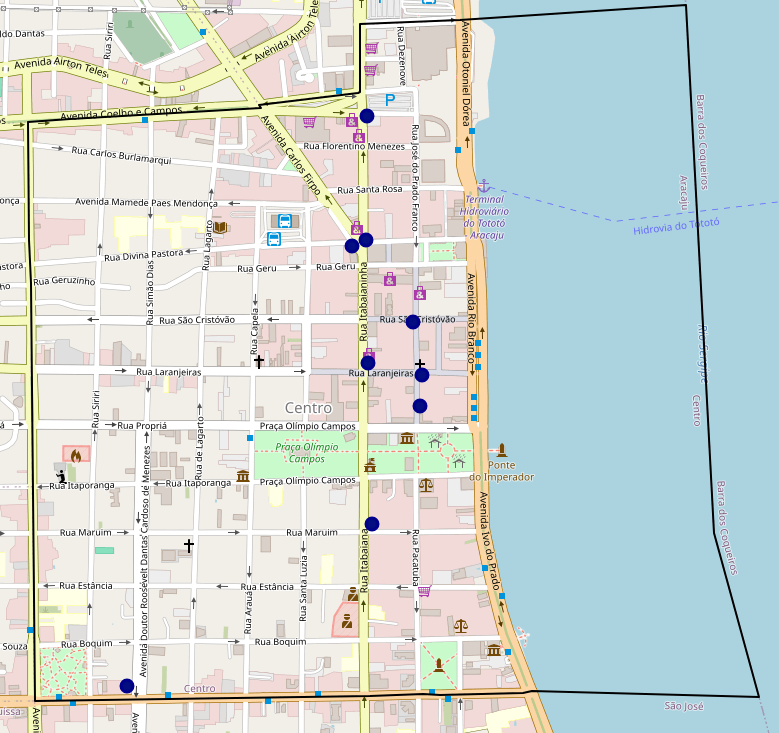
\includegraphics[width=0.6\linewidth]{Artigo/map-farmacias-loc.png}
    \caption{Localização das farmácias no Centro de Aracaju identificadas no OSM.}
    \label{fig:loc-farmacias}
\end{figure}

\begin{figure}[H]
    \centering
    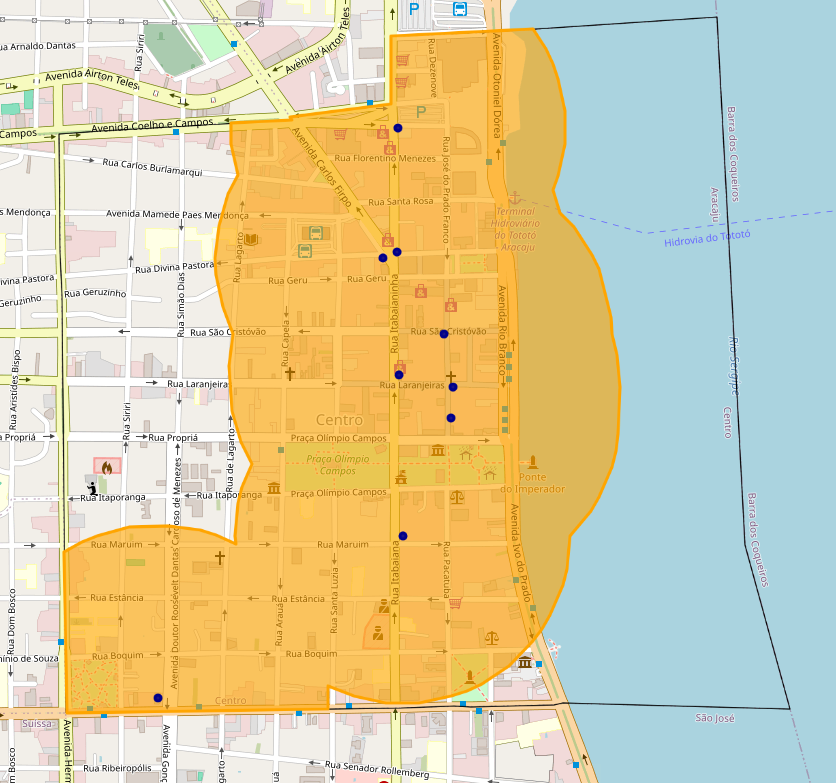
\includegraphics[width=0.6\linewidth]{Artigo/map-farmacias-cobertura.png}
    \caption{Faixas de cobertura das farmácias com raio de 400\,m.}
    \label{fig:cobertura-farmacias}
\end{figure}

\subsection{Análise qualitativa}

Ao analisar a Figura~\ref{fig:cobertura-farmacias} é possível perceber as seguintes situações:

\begin{itemize}
    \item \textbf{Concentração central:} há sobreposição significativa das faixas de cobertura na porção central do bairro, indicando elevada oferta e redundância de serviços nessa área.
    \item \textbf{Lacunas:} nas regiões mais afastadas do núcleo observa-se ausência de cobertura, sinalizando menores níveis de acessibilidade sob o critério adotado (400\,m).
    \item \textbf{Padrão espacial da oferta:} a distribuição das farmácias tende a se concentrar na região com um maior fluxo comercial, comportamento compatível com decisões que visam reduzir a distância entre o estabelecimento e os clientes.
\end{itemize}

\subsection{Interpretação comparativa: PLMC vs. P-Medianas}

Comparando as duas abordagens conceituais aplicadas ao mesmo conjunto de dados, verifica-se o seguinte:

\begin{itemize}
    \item O \emph{PLMC} enfatiza a expansão da fração de demanda coberta em um raio predefinido; em cenários com \(P\) restrito e \(d\) curto, a tendência é dispersar instalações para reduzir lacunas de atendimento.
    \item O modelo das P-Medianas privilegia a minimização da distância média de deslocamento, o que tende a concentrar instalações em áreas de maior densidade de demanda, aumentando a eficiência média de deslocamento, porém potencialmente deixando zonas mais distantes descobertas.
    \item No caso estudado, a configuração observada das farmácias aproxima-se mais da lógica das P-Medianas: há prioridade na redução das distâncias médias, com consequente presença de lacunas de cobertura em áreas mais remotas.
\end{itemize}

\section{Conclusão}
Em síntese, os resultados deste estudo sugerem que a disposição atual das farmácias no Centro de Aracaju favorece a \emph{acessibilidade média} em detrimento da \emph{cobertura máxima} no raio considerado (400\,m). Contudo, tais conclusões são preliminares e limitadas por certas restrições metodológicas:

\begin{itemize}
    \item O raio de cobertura adotado (400\,m) é arbitrário e não considera diferentes modais de transporte, o que pode afetar a interpretação dos resultados.
    \item A análise foi exploratória e não incluiu simulações estocásticas ou otimizações formais, o que reduz a robustez das conclusões.
\end{itemize}

Recomenda-se que estudos futuros acerca do cenário elaborado expandam o escopo da aplicação através das seguintes proposições:
\begin{itemize}
    \item Realizar avaliação conjunta dos dois modelos, examinando possível trade-offs entre o número de farmácias e a distância média dos clientes, incluindo variáveis socioeconômicas e fluxos de demanda para formalizar uma decisão de planejamento.
    \item Explorem outras formulações de localização, como, CFLP ou TUFLP, por exemplo, e considerem a inclusão de novos elos da cadeia farmacêutica, distribuidoras e clínicas, para ampliar a abrangência da análise.
\end{itemize}

\begin{thebibliography}{99}

\bibitem{SousaFilho2012} FILHO, G. S. et al. Uma arquitetura e ferramentas para problemas de localização de facilidades no setor público. São Paulo: SBC, 2012. Disponível em: <https://sol.sbc.org.br/index.php/sbsi/article/view/14428>

\bibitem{Rushton1979} RUSHTON, G. Optimal Location of Facilities. [s.l.] Department of Geography, University of Iowa, jan. 1979.

\bibitem{KuoKung2025} KUNG, L.-C.; CHUANG, J.-S.; KUO, Y.-T. Optimal Allocation of Capacitated Facilities considering Time-dependent User Preference for User Number Maximization. Disponível em: <https://ssrn.com/abstract=4276750>. Acesso em: 5 set. 2025. 

\bibitem{Busing2024} BÜSING, C.; GERSING, T.; WREDE, S. Insights into the computational complexity of the single-source capacitated facility location problem with customer preferences. [s.l.] Optimization Online, dez. 2024. 

\bibitem{Kang2023} KANG, C.-N. et al. A service facility location problem considering customer preference and facility capacity. Computers \& Industrial Engineering, v. 177, p. 109070, 2023.

\bibitem{OwenDaskin1998} OWEN, S. H.; DASKIN, M. S. Strategic facility location: A review. European Journal of Operational Research, v. 111, p. 423–447, 1998. 

\bibitem{Alarcon-GerbierBuscher2022} ALARCONGERBIER, E.; BUSCHER, U. Modular and mobile facility location problems: A systematic review. Computers \& Industrial Engineering, v. 173, p. 108734, 2022. 

\bibitem{ChurchReVelle2010} CHURCH, R.; REVELLE, C. Theoretical and Computational Links between the pMedian, Location Setcovering, and the Maximal Covering Location Problem. Geographical Analysis, v. 8, p. 406–415, 3 set. 2010. 

\bibitem{Pedroso2012} PEDROSO, J. P. et al. Facility Location Problems — Mathematical Optimization: Solving Problems Using Gurobi and Python. Disponível em: <https://scipbook.readthedocs.io/en/latest/flp.html>.

\end{thebibliography}

\end{document}